\documentclass[tikz, border = 10pt]{standalone}

\renewcommand{\familydefault}{\sfdefault} 

\usetikzlibrary{positioning, quotes, calc, arrows.meta, bending, shapes, backgrounds}

\tikzset{
every node/.style = {scale = 1.1},
manifest/.style = {rectangle, draw, thin, inner sep = 5pt, minimum width = 1cm, 
	minimum height = 1cm},
latent/.style = {ellipse, draw, thin, inner sep = 5pt, minimum width = 1cm, 
	minimum height = 1cm},
residual1/.style = {circle, draw, thin, minimum size = 5mm, inner sep = 1pt}, 
residual2/.style = {rectangle, minimum width = 0.5pt, minimum height = 1.5mm, 
	inner sep = 0pt, outer sep = 0mm},
regression/.style = {-{Stealth[length = 1.5mm]}, thin, shorten > = 1pt, inner sep = 2pt},
covariance/.style={{Stealth[length = 1.5mm]}-{Stealth[length = 1.5mm]}, thin, 
	shorten > = 1pt, shorten < = 1pt, inner sep = 2pt},
variance/.style={{Stealth[length = 1mm]}-{Stealth[length = 1mm]}, thin, 
	shorten > = 1pt, shorten < = 1pt, inner sep = 1.5pt},
interaction/.style = {-{Stealth[sep = 1pt, length = 1.5mm] . Circle[length = 4pt]}, 
	thin, shorten > = -2pt},
constant/.style = {draw, thin, inner sep = 1pt, regular polygon, 
    regular polygon sides = 3, minimum size = 5mm}
}

\begin{document}
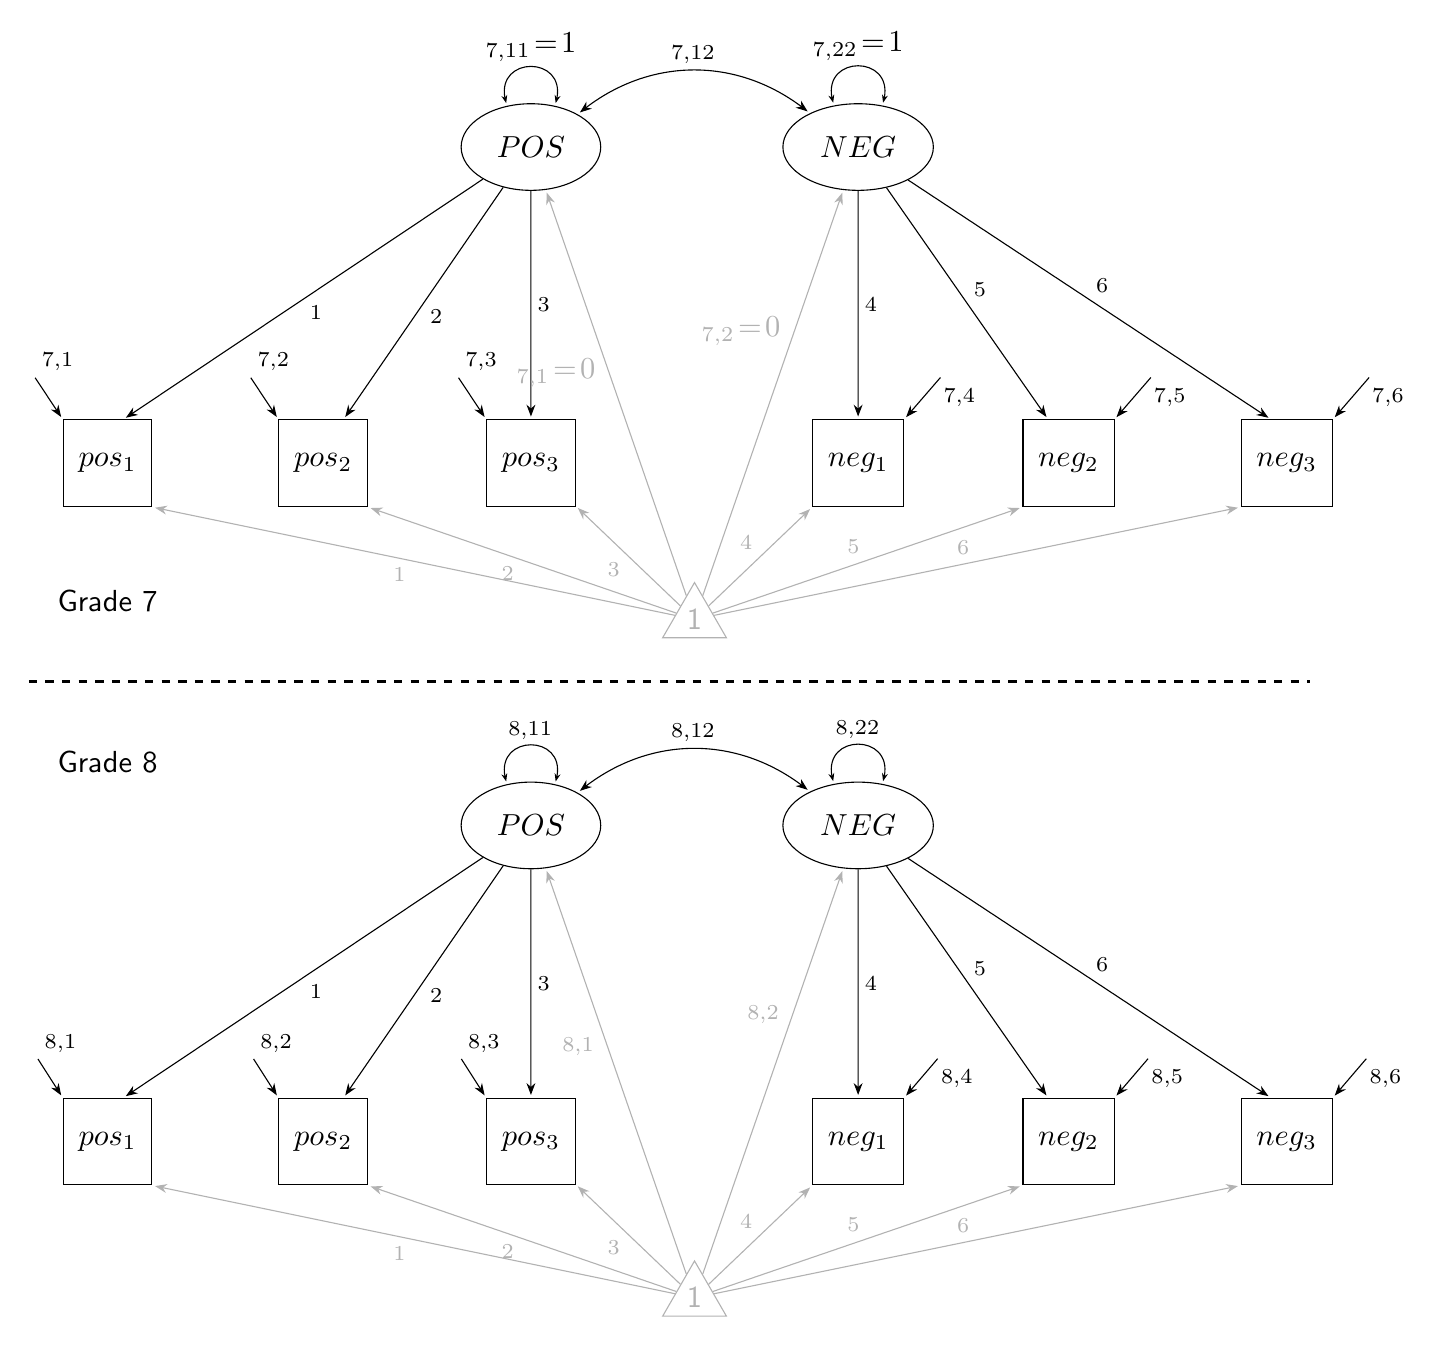
\begin{tikzpicture}

%%%% Grade 7
%% pos manifests
\node [manifest] (pos71) {$pos_1$};
\node [manifest] (pos72) [right = 1.6cm of pos71] {$pos_2$};
\node [manifest] (pos73) [right = 1.5cm of pos72] {$pos_3$};

%% neg manifests
\node [manifest] (neg71) [right = 3cm of pos73] {$neg_1$};
\node [manifest] (neg72) [right = 1.5cm of neg71] {$neg_2$};
\node [manifest] (neg73) [right = 1.6cm of neg72] {$neg_3$};

%% POS and NEG latents
\node [latent] (POS7) [above = 2.9cm of pos73] {$POS$};
\node [latent] (NEG7) [above = 2.9cm of neg71] {$NEG$};

%% Loadings
\path [regression] (POS7) edge ["$\uplambda_1$"] (pos71.70);
\path [regression] (POS7) edge ["$\uplambda_2$"] (pos72.65);
\path [regression] (POS7) edge ["$\uplambda_3$"] (pos73.90);

\path [regression] (NEG7) edge ["$\uplambda_4$"] (neg71.90);
\path [regression] (NEG7) edge ["$\uplambda_5$"] (neg72.115);
\path [regression] (NEG7) edge ["$\uplambda_6$"] (neg73.110);

%% Latent variances ans covariance
\path [covariance] (POS7.35) edge ["$\upphi_{7,12}$", bend left = 40] (NEG7.145);
\path [variance] (POS7.120) edge ["$\upphi_{7,11}\!=\!1$", above, bend left = 110, looseness = 3] (POS7.60);
\path [variance] (NEG7.120) edge ["$\upphi_{7,22}\!=\!1$", above, bend left = 110, looseness = 3] (NEG7.60);

%% Residuals
\node [residual2] (e71) [above left = .65cm of pos71, xshift = 1mm] {};
\path [regression] (e71) edge ["$\uptheta_{7,1}$", pos = 0] (pos71.north west);

\node [residual2] (e72) [above left = .65cm of pos72, xshift = 1mm] {};
\path [regression] (e72) edge ["$\uptheta_{7,2}$", pos = 0] (pos72.north west);

\node [residual2] (e73) [above left = .65cm of pos73, xshift = 1mm] {};
\path [regression] (e73) edge ["$\uptheta_{7,3}$", pos = 0] (pos73.north west);

\node [residual2] (e74) [above right = .65cm of neg71] {};
\path [regression] (e74) edge ["$\uptheta_{7,4}$", pos = 0.1] (neg71.north east);

\node [residual2] (e75) [above right = .65cm of neg72] {};
\path [regression] (e75) edge ["$\uptheta_{7,5}$", pos = 0.1] (neg72.north east);

\node [residual2] (e76) [above right = .65cm of neg73] {};
\path [regression] (e76) edge ["$\uptheta_{7,6}$", pos = 0.1] (neg73.north east);

%% latent means
\node [constant, black!30] (M7) [below = 1.5cm of $(pos73)!0.5!(neg71)$] {1};
\path [regression, black!30] (M7) edge ["$\upkappa_{7,1}\!=\!0$", pos = .6] (POS7);
\path [regression, black!30] (M7) edge ["$\upkappa_{7,2}\!=\!0$", pos = .6] (NEG7);

%% Intercepts
\path [regression, black!30] (M7) edge ["$\uptau_1$"] (pos71.south east);
\path [regression, black!30] (M7) edge ["$\uptau_2$"] (pos72.south east);
\path [regression, black!30] (M7) edge ["$\uptau_3$"] (pos73);

\path [regression, black!30] (M7) edge ["$\uptau_4$"] (neg71);
\path [regression, black!30] (M7) edge ["$\uptau_5$"] (neg72.south west);
\path [regression, black!30] (M7) edge ["$\uptau_6$"] (neg73.south west);


%%%% Grade 8 %%%%%%%%%%%
%% pos manifests
\node [manifest] (pos81) [below = 7.5cm of pos71] {$pos_1$};
\node [manifest] (pos82) [right = 1.6cm of pos81] {$pos_2$};
\node [manifest] (pos83) [right = 1.5cm of pos82] {$pos_3$};

%% neg manifests
\node [manifest] (neg81) [right = 3cm of pos83] {$neg_1$};
\node [manifest] (neg82) [right = 1.5cm of neg81] {$neg_2$};
\node [manifest] (neg83) [right = 1.6cm of neg82] {$neg_3$};

%% POS and NEG latents
\node [latent] (POS8) [above = 2.9cm of pos83] {$POS$};
\node [latent] (NEG8) [above = 2.9cm of neg81] {$NEG$};

%% Loadings
\path [regression] (POS8) edge ["$\uplambda_1$"] (pos81.70);
\path [regression] (POS8) edge ["$\uplambda_2$"] (pos82.65);
\path [regression] (POS8) edge ["$\uplambda_3$"] (pos83.90);

\path [regression] (NEG8) edge ["$\uplambda_4$"] (neg81.90);
\path [regression] (NEG8) edge ["$\uplambda_5$"] (neg82.115);
\path [regression] (NEG8) edge ["$\uplambda_6$"] (neg83.110);

%% Latent variances ans covariance
\path [covariance] (POS8.35) edge ["$\upphi_{8,12}$", bend left = 40] (NEG8.145);
\path [variance] (POS8.120) edge ["$\upphi_{8,11}$", above, bend left = 110, looseness = 3] (POS8.60);
\path [variance] (NEG8.120) edge ["$\upphi_{8,22}$", above, bend left = 110, looseness = 3] (NEG8.60);

%% Residuals
\node [residual2] (e81) [above left = .6cm of pos81, xshift = 1mm] {};
\path [regression] (e81) edge ["$\uptheta_{8,1}$", pos = 0] (pos81.north west);

\node [residual2] (e82) [above left = .6cm of pos82, xshift = 1mm] {};
\path [regression] (e82) edge ["$\uptheta_{8,2}$", pos = 0] (pos82.north west);

\node [residual2] (e83) [above left = .6cm of pos83, xshift = 1mm] {};
\path [regression] (e83) edge ["$\uptheta_{8,3}$", pos = 0] (pos83.north west);

\node [residual2] (e84) [above right = .6cm of neg81] {};
\path [regression] (e84) edge ["$\uptheta_{8,4}$", pos = 0.1] (neg81.north east);

\node [residual2] (e85) [above right = .6cm of neg82] {};
\path [regression] (e85) edge ["$\uptheta_{8,5}$", pos = 0.1] (neg82.north east);

\node [residual2] (e86) [above right = .6cm of neg83] {};
\path [regression] (e86) edge ["$\uptheta_{8,6}$", pos = 0.1] (neg83.north east);

%% latent means
\node [constant, black!30] (M8) [below = 1.5cm of $(pos83)!0.5!(neg81)$] {1};
\path [regression, black!30] (M8) edge ["$\upkappa_{8,1}$", pos = .6] (POS8);
\path [regression, black!30] (M8) edge ["$\upkappa_{8,2}$", pos = .6] (NEG8);

%% Intercepts
\path [regression, black!30] (M8) edge ["$\uptau_1$"] (pos81.south east);
\path [regression, black!30] (M8) edge ["$\uptau_2$"] (pos82.south east);
\path [regression, black!30] (M8) edge ["$\uptau_3$"] (pos83);

\path [regression, black!30] (M8) edge ["$\uptau_4$"] (neg81);
\path [regression, black!30] (M8) edge ["$\uptau_5$"] (neg82.south west);
\path [regression, black!30] (M8) edge ["$\uptau_6$"] (neg83.south west);


\node (gp1) at (0,-1.75) {Grade 7};
\node (gp2) [below = 1.5cm of gp1] {Grade 8};

\node (C1) at ($(gp1)!0.5!(gp2)$) {};
\node (C2) [right = 14cm of C1] {};
\draw[dashed, thick] ($(C1)!-1cm!(C2)$) -- ($(C2)!-1cm!(C1)$);

\end{tikzpicture}
\end{document}





